%!TEX program = xelatex
\documentclass[en,hazy,cyan,8pt,normal]{elegantnote}
\title{SUSTech - 25Fall - MAE5009 - Note}

\author{Yiyuan YING}
\institute{Southern University of Science and Technology}

% \version{2.50}
\date{\today}

\usepackage{array}
\usepackage{float}
\usepackage{microtype} % 微排版,通常能减少 underfull/overfull
\usepackage{amsmath}   % 数学公式排版包
\usepackage{hyperref}  % hyperref需要在cleveref之前加载
\usepackage{cleveref}  % 添加智能引用宏包

% 修改公式编号格式为"章节号-公式序号"
\numberwithin{equation}{section}
\renewcommand{\theequation}{\thesection-\arabic{equation}}

% 自定义cleveref的引用格式 - 使用英文缩写格式
\crefname{equation}{Eq.}{Eqs.}
\Crefname{equation}{Equation}{Equations}
\crefname{figure}{Fig.}{Figs.}
\Crefname{figure}{Figure}{Figures}
\crefname{table}{Tab.}{Tabs.}
\Crefname{table}{Table}{Tables}
\crefname{section}{Sec.}{Secs.}
\Crefname{section}{Section}{Sections}
\crefname{subsection}{Sec.}{Secs.}
\Crefname{subsection}{Subsection}{Subsections}

% 修复引用格式问题 - 确保引用显示完整的编号格式
\creflabelformat{equation}{#2(#1)#3}

\begin{document}

\maketitle

\section{Stress Analysis}
  \subsection{Stress State}
    \begin{itemize}
      \item Normal Stress
      \item Shear Stress
      \item Stress Transformation
    \end{itemize}

  \subsection{Equilibrium Equation of Stress}
    \begin{itemize}
      \item Body Force: Gravitational Force, Magnetic Force, Inertial Force
      \item Surface Force: Friction Force, Pressure, Viscous Force(Fluid Flow)
    \end{itemize}

    \begin{equation}\label{eq:001}
      \sigma=\lim_{\Delta A \to 0} \frac{\Delta F}{\Delta A}
    \end{equation}

    The equation means the force at the per unit surface area. The unit is Pascal($Pa=N/m^2$).

    Other common units:
    \begin{itemize}
      \item $1 atm \approx 10^5 Pa = 0.1 MPa$
      \item $1 bar \approx 0.98 atm \approx 1 atm = 0.1 MPa$
    \end{itemize}

    Stress is a kind of tensor, different from \textbf{scalar} and \textbf{vector}.
    \begin{itemize}
      \item Scalar: only have magnitude, e.g. temperature, density;
      \item Vector: have both magnitude and direction, e.g. velocity, force;
      \item Tensor: magnitude and direction in multiple directions, e.g. stress, strain.
    \end{itemize}

    At a reference plane, the force $F$ is vertically upward, the normal stress $\sigma$ is perpendicular to the plane, while the shear stress $\tau$ is parallel to the plane.

  \subsection{2D Stress}
    \begin{figure}[H]
      \centering
      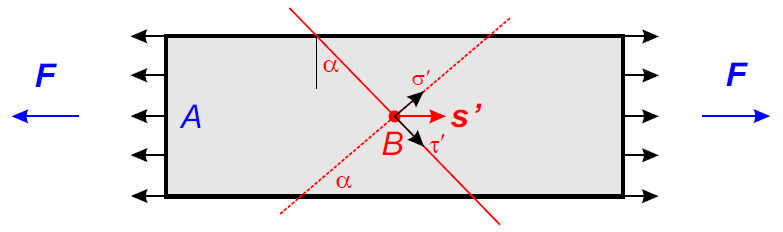
\includegraphics[width=0.6\textwidth]{image/001.png}
      \caption{Stress components on a reference plane}
      \label{fig:001}
    \end{figure}

    For the circumstances shown in \cref{fig:001}, the normal stress and shear stress on the reference plane can be determined.

    \begin{equation}\label{eq:002}
      A'=\frac{A}{\sin \alpha}, \quad S=\frac{F}{A'}=\frac{F}{A} \sin \alpha,\quad
      \left\{
      \begin{aligned}
        \tau&=S\cdot\cos\alpha=\frac{F}{A} \sin \alpha \cos \alpha\\
        \sigma&=S\cdot\sin\alpha=\frac{F}{A} \sin^2 \alpha
      \end{aligned}
      \right.
    \end{equation}

  \subsection{3D Stress}
    \begin{figure}[H]
      \centering
      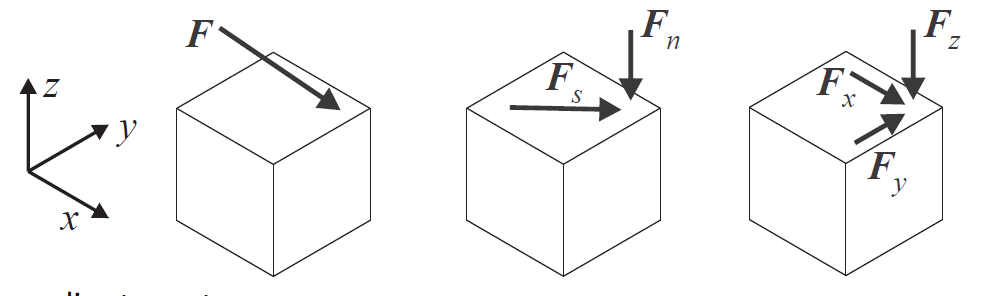
\includegraphics[width=0.6\textwidth]{image/002.png}
      \caption{Decomposition of an external force$F$}
      \label{fig:002}
    \end{figure}

    As shown in \cref{fig:002}, the force $F$ applied at an arbitrary angle to the x-y plane can be resolved into a normal component $F_n$ and a shear component $F_s$. The shear component can be further decomposed into Cartesian components $F_x$ and $F_y$.

    \begin{figure}[H]
      \centering
      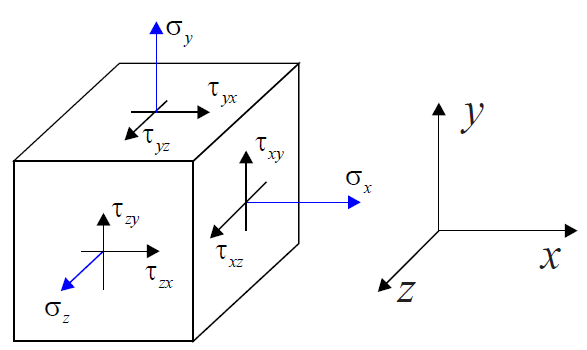
\includegraphics[width=0.6\textwidth]{image/003.png}
      \caption{Three-Dimensional State of Stress}
      \label{fig:003}
    \end{figure}

    As shown in the \cref{fig:003}, in every face has three stress components, with 1 normal stress($\sigma_x, \sigma_y, \sigma_z$) and 2 shear stresses($\tau_{xy}, \tau_{xz}, \tau_{yx}, \tau_{yz}, \tau_{zx}, \tau_{zy}$). Thus the components of stress can be expressed in a matrix form:

    \begin{equation}\label{eq:003}
      [\sigma]=
      \begin{bmatrix}
        \sigma_x & \tau_{xy} & \tau_{xz}\\
        \tau_{yx} & \sigma_y & \tau_{yz}\\
        \tau_{zx} & \tau_{zy} & \sigma_z
      \end{bmatrix}
    \end{equation}

    The sign convention is that normal stresses causing tension are positive, while those causing compression are negative.
    If we consider rotational equilibrium of the infinitesimal square shown as \cref{fig:004}, we can calculate the moment with respect to lower left corner:

    \begin{figure}[H]
      \centering
      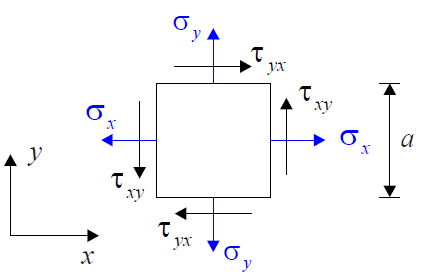
\includegraphics[width=0.4\textwidth]{image/004.png}
      \caption{Rotational Equilibrium of an Infinitesimal Element}
      \label{fig:004}
    \end{figure}

    \begin{equation}\label{eq:004}
      \sigma_x\cdot a (a/2)-\sigma_x\cdot a (a/2)+\sigma_y\cdot a (a/2)-\sigma_y\cdot a (a/2)+\tau_{xy}\cdot a \cdot a - \tau_{yx}\cdot a \cdot a=0
    \end{equation}

    Thus we have:

    \begin{equation}\label{eq:005}
      \tau_{xy}=\tau_{yx}
    \end{equation}

    Similarly, we can have:

    \begin{equation}\label{eq:006}
      \tau_{yz}=\tau_{zy}, \tau_{zx}=\tau_{xz}
    \end{equation}

    Which means, the stress matrix is symmetric, and there are 3 normal stresses and 3 shear stresses, totally 6 independent stress components in 3D stress state.

    \begin{equation}\label{eq:007}
      [\sigma]=
      \begin{bmatrix}
        \sigma_x & \tau_{xy} & \tau_{xz}\\
          & \sigma_y & \tau_{yz}\\
        Sym. &   & \sigma_z
      \end{bmatrix}
    \end{equation}

  \subsection{2D Stress Transformation}
    \begin{figure}[H]
      \centering
      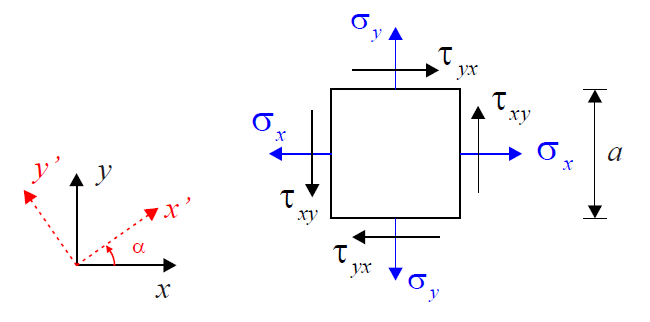
\includegraphics[width=0.6\textwidth]{image/005.png}
      \caption{Stress Transformation on an Arbitrary Plane}
      \label{fig:005}
    \end{figure}

    \begin{figure}[H]
      \centering
      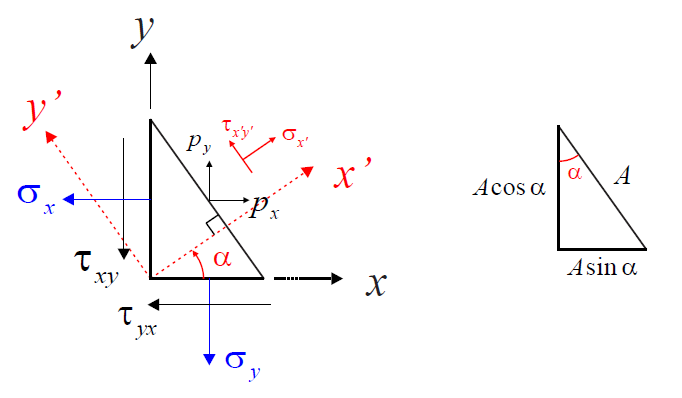
\includegraphics[width=0.6\textwidth]{image/006.png}
      \caption{Stress Components on an Inclined Plane in 2D Stress State}
      \label{fig:006}
    \end{figure}

    After the transformation shown in \cref{fig:005}, the new stress components are shown in \cref{fig:006}.
    The stress transformation equations may be derived based on force equilibrium analysis:

    \begin{equation}\label{eq:008}
      \sum F_x=0\Rightarrow p_x=\sigma_x\cos\alpha+\tau_{yx}\sin\alpha
    \end{equation}

    \begin{equation}\label{eq:009}
      \sum F_y=0\Rightarrow p_y=\sigma_y\sin\alpha+\tau_{xy}\cos\alpha
    \end{equation}

    Thus we have:

    \begin{equation}\label{eq:010}
      \left\{
      \begin{aligned}
        \sigma_{x'}&=\frac{\sigma_x+\sigma_y}{2}+\frac{\sigma_x-\sigma_y}{2}\cos2\alpha+\tau_{xy}\sin2\alpha\\
        \sigma_{y'}&=\frac{\sigma_x+\sigma_y}{2}-\frac{\sigma_x-\sigma_y}{2}\cos2\alpha-\tau_{xy}\sin2\alpha\\
        \tau_{x'y'}&=-\frac{\sigma_x-\sigma_y}{2}\sin2\alpha+\tau_{xy}\cos2\alpha
      \end{aligned}
      \right.
    \end{equation}

    In 2D circumstances, $\sigma'$ can be calculated by $\sigma'=\mathbf{R}\sigma \mathbf{R}^T$, in which:

    \begin{equation}\label{eq:011}
      \sigma=
      \begin{bmatrix}
        \sigma_x & \tau_{yx}\\
        \tau_{xy} & \sigma_y
      \end{bmatrix}, 
      \mathbf{R}=
      \begin{bmatrix}
        \cos\alpha & \sin\alpha\\
        -\sin\alpha & -\cos\alpha
      \end{bmatrix},
      \sigma'=
      \begin{bmatrix}
        \sigma_x' & \tau_{yx}'\\
        \tau_{xy}' & \sigma_y'
      \end{bmatrix}
    \end{equation}

    Also, the rotation angle $\alpha$ (principle directions)can be calculated by:

    \begin{equation}\label{eq:012}
      \tan2\alpha=\frac{2\tau_{xy}}{\sigma_x-\sigma_y}(\alpha\in[0,\pi])
    \end{equation}

    \begin{equation}\label{eq:013}
      \sin2\alpha=\pm\frac{2\tau_{xy}}{\sqrt{4\tau_{xy}^2+(\sigma_x-\sigma_y)^2}}, \quad \cos2\alpha=\frac{\sigma_x-\sigma_y}{\sqrt{4\tau_{xy}^2+(\sigma_x-\sigma_y)^2}}
    \end{equation}

    The principle stress can be calculated by:

    \begin{equation}\label{eq:014}
      \sigma_{1}=\frac{\sigma_x+\sigma_y}{2} + \sqrt{\left(\frac{\sigma_x-\sigma_y}{2}\right)^2+\tau_{xy}^2}
    \end{equation}

    \begin{equation}\label{eq:015}
      \sigma_{2}=\frac{\sigma_x+\sigma_y}{2} - \sqrt{\left(\frac{\sigma_x-\sigma_y}{2}\right)^2+\tau_{xy}^2}
    \end{equation}

    \begin{equation}\label{eq:016}
      \tau_{x'y'max}=\pm\sqrt{\left(\frac{\sigma_x-\sigma_y}{2}\right)^2+\tau_{xy}^2}
    \end{equation}
  
  \subsection{Mohr's circle of stress}
    \begin{figure}[H]
      \centering
      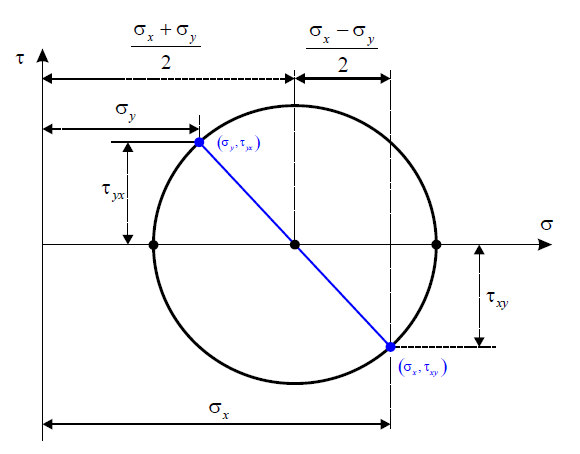
\includegraphics[width=0.6\textwidth]{image/007.png}
      \caption{Mohr's Circle of Stress}
      \label{fig:007}
    \end{figure}

    As shown in the \cref{fig:007}, 2D stress transformation can also be conveniently represented graphically in a circle. And from \cref{eq:010}, we can calculate that the equation of the circle is:

    \begin{equation}\label{eq:017}
      \left( \sigma - \frac{\sigma_x + \sigma_y}{2} \right)^2 + \tau^2 = \left( \frac{\sigma_x - \sigma_y}{2} \right)^2 + \tau_{xy}^2
    \end{equation}

    From the \cref{eq:017} we can get the center is $\displaystyle \left(\frac{\sigma_x + \sigma_y}{2}, 0\right)$ and the radius is $\displaystyle R=\sqrt{\left( \frac{\sigma_x - \sigma_y}{2} \right)^2 + \tau_{xy}^2}$.

    \begin{figure}[H]
      \centering
      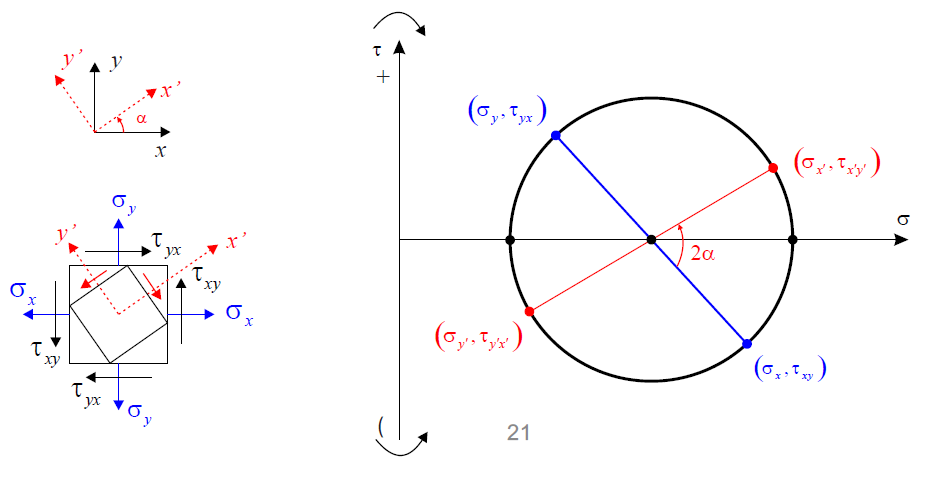
\includegraphics[width=0.6\textwidth]{image/008.png}
      \caption{Rotation in the Mohr's Circle of Stress}
      \label{fig:008}
    \end{figure}

    After rotating the x-y axis as shown in the \cref{fig:008}, the stress would be:

    \begin{equation}\label{eq:018}
      \left\{
      \begin{aligned}
        \sigma_x'&=\frac{\sigma_1+\sigma_2}{2}+\frac{\sigma_1-\sigma_2}{2}\cos2\alpha\\
        \sigma_y'&=\frac{\sigma_1+\sigma_2}{2}-\frac{\sigma_1-\sigma_2}{2}\cos2\alpha\\
        \tau_{x'y'}&=-\frac{\sigma_1-\sigma_2}{2}\sin2\alpha
      \end{aligned}
      \right.
    \end{equation}
  
  \subsection{3D stress transformation}
    Same to 2D stress transformation, the 3D stress transformation can also be expressed in matrix form:

    \begin{equation}\label{eq:019}
      \sigma'=\mathbf{R}\sigma \mathbf{R}^T
    \end{equation}

    where

    \begin{equation}\label{eq:020}
      \mathbf{R} =
        \begin{bmatrix}
        a_{11} & a_{12} & a_{13} \\
        a_{21} & a_{22} & a_{23} \\
        a_{31} & a_{32} & a_{33}
        \end{bmatrix}
        =
        \begin{bmatrix}
        \cos(x', x) & \cos(x', y) & \cos(x', z) \\
        \cos(y', x) & \cos(y', y) & \cos(y', z) \\
        \cos(z', x) & \cos(z', y) & \cos(z', z)
        \end{bmatrix}
    \end{equation}

    which means the direction cosines between the old and new coordinate axes.
    And in each columns and rows of matrix $\mathbf{R}$, we have:

    \begin{equation}\label{eq:021}
      a_{1i}^2 + a_{2i}^2 + a_{3i}^2 = 1, \quad i=1,2,3
    \end{equation}

    \begin{equation}\label{eq:022}
      a_{i1}^2 + a_{i2}^2 + a_{i3}^2 = 1, \quad i=1,2,3
    \end{equation}

  \subsection{3D principal stress}
    For symmetric matrix $\mathbf{A}$, its eigenvalue and eigenvector satisfy:

    \begin{equation}\label{eq:023}
      \mathbf{A}\mathbf{v}=\lambda \mathbf{v}
    \end{equation}

    \begin{equation}\label{eq:024}
      (\mathbf{A}-\lambda \mathbf{I})\mathbf{v}=0
    \end{equation}

    As the equation has non-zero $\mathbf{v}$ if and only if:

    \begin{equation}\label{eq:025}
      |\mathbf{A}-\lambda \mathbf{I}|=0
    \end{equation}

    Then we have the \textbf{Characteristic Equation} for the principle stress(in \cref{eq:023,eq:024,eq:025}, the matrix $\mathbf{A}$ can be replaced by stress matrix $[\sigma]$):

    \begin{equation}\label{eq:026}
      \det(\mathbf{\sigma}-\lambda \mathbf{I})=0
    \end{equation}

    Expand the determinant, we have:

    \begin{equation}\label{eq:027}
      \lambda^3 - I_1 \lambda^2 + I_2 \lambda - I_3 = 0
    \end{equation}

    The invariants $I_1, I_2, I_3$ are \textbf{Stress Invariants}, which means they are independent of the coordinate system:

    \begin{equation}\label{eq:028}
      \begin{cases}
        I_1 = \sigma_x + \sigma_y + \sigma_z=\sigma_1 + \sigma_2 + \sigma_3\\
        I_2 = \sigma_x \sigma_y + \sigma_y \sigma_z + \sigma_z \sigma_x - \tau_{xy}^2 - \tau_{yz}^2 - \tau_{zx}^2 = \sigma_1 \sigma_2 + \sigma_2 \sigma_3 + \sigma_3 \sigma_1\\
        I_3 = \sigma_x \sigma_y \sigma_z + 2 \tau_{xy} \tau_{yz} \tau_{zx} - \sigma_x \tau_{yz}^2 - \sigma_y \tau_{zx}^2 - \sigma_z \tau_{xy}^2 = \sigma_1 \sigma_2 \sigma_3
      \end{cases}
    \end{equation}

  \subsection{Differential equation of equilibrium}
    \begin{figure}[H]
      \centering
      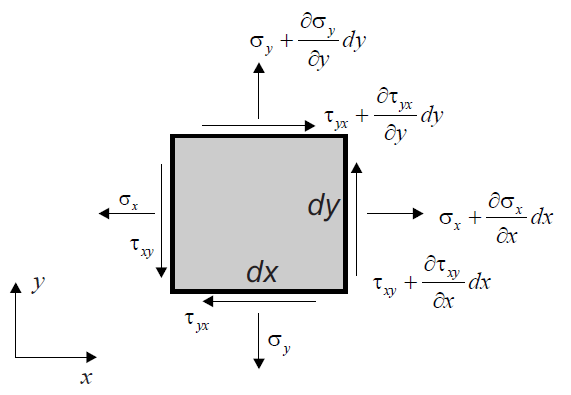
\includegraphics[width=0.6\textwidth]{image/009.png}
      \caption{Differential Element under Stress and Body Force}
      \label{fig:009}
    \end{figure}

    For the force balance $\sum F=0$ in the circumstances shown in \cref{fig:009}, we have:

    \begin{equation}\label{eq:029}
      \left\{
      \begin{aligned}
        \displaystyle \frac{\partial\sigma_x}{\partial x}+\frac{\partial\tau_{yx}}{\partial y}+\frac{\partial\tau_{zx}}{\partial z}+f_x=0 \\
        \displaystyle \frac{\partial\tau_{xy}}{\partial x}+\frac{\partial\sigma_y}{\partial y}+\frac{\partial\tau_{zy}}{\partial z}+f_y=0 \\
        \displaystyle \frac{\partial\tau_{xz}}{\partial x}+\frac{\partial\tau_{yz}}{\partial y}+\frac{\partial\sigma_z}{\partial z}+f_z=0
      \end{aligned}
      \right.
    \end{equation}

    Which can be expressed like:

    \begin{equation}\label{eq:030}
      \nabla \cdot \sigma + f = 0
    \end{equation}

    In the \cref{eq:029,eq:030}, $f$ is the body force intensities(per unit volume), e.g. gravitational force, magnetic force, inertial force.

    And when the body has acceleration, the \cref{eq:030} can be expressed as:

    \begin{equation}\label{eq:031}
      \nabla \cdot \sigma + f = \rho \frac{\partial^2 u}{\partial t^2}
    \end{equation}

    And for the torque balance $\sum M=0$ in the circumstances shown in \cref{fig:009}, we have:

    \begin{equation}\label{eq:032}
        \tau_{xy}=\tau_{yx}, \tau_{yz}=\tau_{zy}, \tau_{zx}=\tau_{xz}
    \end{equation}

    From the \cref{eq:029}, there are 6 independent unkowns in total, while only 3 equations. Thus additional equations are needed to complete the solutions of the stress distribution in a body. For example, Strain-displacement, Generalized Hooke's Law, etc.

\section{Strain Analysis}

  \subsection{Assumptions}
    \begin{itemize}
      \item Infinitesimal deformation (1\% - 5\%)
      \item Continuous materials
      \begin{itemize}
        \item Continuous displacement
        \item No gap/discontinuities after displacement
      \end{itemize}
      \item Displacement functions must be single-valued
    \end{itemize}

  \subsection{Strain \& Displacement}
    Same to stress, strain also can be devided into:

    \begin{itemize}
      \item \textbf{Normal Strain}: relative changes of the \textbf{length} of the objects
      \item \textbf{Shear Strain}: changes of the \textbf{angle} of the two sides of the objects
    \end{itemize}

    And the definition of the strain is:

    \begin{equation}\label{eq:033}
      \varepsilon=\frac{\Delta L}{L}
    \end{equation}

    which is dimensionless.

    \begin{figure}[H]
      \centering
      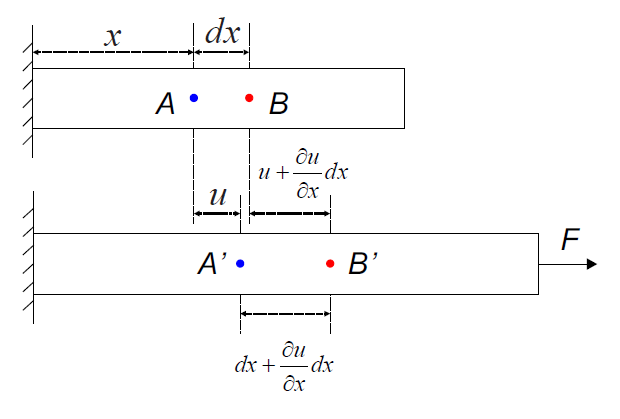
\includegraphics[width=0.6\textwidth]{image/010.png}
      \caption{Deformation of a body under load $F$}
      \label{fig:010}
    \end{figure}

    As shown in \cref{fig:010}, under the load $F$, the strain $\varepsilon$ can be calculated by:

    \begin{equation}\label{eq:034}
      \varepsilon
      =\frac{A'B'-AB}{AB}
      =\frac{dx+\frac{\partial u}{\partial x}dx - dx}{dx}
      =\frac{\frac{\partial u}{\partial x}\cdot dx}{dx}=\frac{\partial u}{\partial x}
    \end{equation}
    
    \begin{figure}[H]
      \centering
      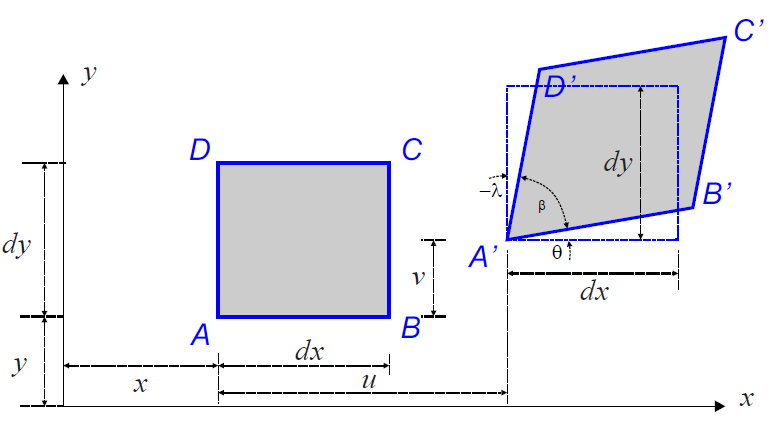
\includegraphics[width=0.6\textwidth]{image/011.png}
      \caption{2D deformation of a body under load}
      \label{fig:011}
    \end{figure}

    As shown in \cref{fig:011}, the normal strain and the shear strain can be calculated by \cref{eq:035,eq:036,eq:037}, and the deformation of the body in both horizontal and vertical can be calculated by \cref{tab:001}.

    \begin{equation}\label{eq:035}
      \varepsilon_x=\frac{A'B'-AB}{AB}=\frac{A'B'-dx}{dx}
    \end{equation}

    \begin{equation}\label{eq:036}
      \varepsilon_y=\frac{A'D'-AD}{AD}=\frac{A'D'-dy}{dy}
    \end{equation}

    \begin{equation}\label{eq:037}
      \gamma=\frac{\pi}{2}-\beta
    \end{equation}

    \begin{table}[H]
      \centering
      \caption{Deformation of a body in 2D}
      \label{tab:001}
      \begin{tabular}{|c|c|c|}
        \hline
          & Horizontal & Vertical \\
        \hline
        A & $u(x,y)$ & $v(x,y)$ \\
        \hline
        B & $u(x,y)+\frac{\partial u}{\partial x}dx$ & $v(x,y)+\frac{\partial v}{\partial x}dx$ \\
        \hline
        D & $u(x,y)+\frac{\partial u}{\partial y}dy$ & $v(x,y)+\frac{\partial v}{\partial y}dy$ \\
        \hline
      \end{tabular}
    \end{table}
    
    From \cref{tab:001}, we can calculate the normal strain and shear strain in 2D:

    \begin{equation}\label{eq:038}
      (A'B')^2 = (dx + \frac{\partial u}{\partial x} dx)^2 + (\frac{\partial v}{\partial x} dx)^2 = (dx(1+\varepsilon_x)^2)\\
      \Rightarrow (1+\varepsilon_x)^2 = (1+\frac{\partial u}{\partial x})^2 + (\frac{\partial v}{\partial x})^2
    \end{equation}

    As $\displaystyle \frac{\partial v}{\partial x}\approx 1\% - 5\%$, we have: $\displaystyle\varepsilon_x=\frac{\partial u}{\partial x}$, and similarly, $\displaystyle\varepsilon_y=\frac{\partial v}{\partial y}$. And for 3D circumstances, we have $\displaystyle\varepsilon_z=\frac{\partial w}{\partial z}$.

    For the defoemation of angle, we have:

    \begin{equation}\label{eq:039}
      \theta\rightarrow 0, \theta = \tan \theta = \frac{\frac{\partial v}{\partial x}dx}{dx + \frac{\partial u}{\partial x}dx} = \frac{\frac{\partial v}{\partial x}}{1 + \frac{\partial u}{\partial x}} = \frac{\partial v}{\partial x}
    \end{equation}

    \begin{equation}\label{eq:040}
      \lambda\rightarrow 0, -\lambda = -\tan\lambda = \frac{\frac{\partial u}{\partial y}dy}{dy + \frac{\partial v}{\partial y}dy} = \frac{\frac{\partial u}{\partial y}}{1 + \frac{\partial v}{\partial y}} = \frac{\partial u}{\partial y}
    \end{equation}

    Thus, the shear strain can be expressed as:

    \begin{equation}\label{eq:041}
      \gamma_{xy}=\frac{\pi}{2} - \beta = \theta + (-\lambda) = \frac{\partial v}{\partial x} + \frac{\partial u}{\partial y}
    \end{equation}

    Generalization to three-dimensional case, we have:

    \begin{equation}\label{eq:042}
      \left\{
      \begin{aligned}
        \displaystyle \varepsilon_x=\frac{\partial u}{\partial x}\\
        \displaystyle \varepsilon_y=\frac{\partial v}{\partial y}\\
        \displaystyle \varepsilon_z=\frac{\partial w}{\partial z}
      \end{aligned}
      \right.
      , \quad
      \left\{
      \begin{aligned}
        \displaystyle \gamma_{xy}=\frac{\partial v}{\partial x} + \frac{\partial u}{\partial y}\\
        \displaystyle \gamma_{yz}=\frac{\partial w}{\partial y} + \frac{\partial v}{\partial z}\\
        \displaystyle \gamma_{zx}=\frac{\partial u}{\partial z} + \frac{\partial w}{\partial x}
      \end{aligned}
      \right.
      , \quad
      \left\{
      \begin{aligned}
        \displaystyle \gamma_{xy}=\gamma_{yx}\\
        \displaystyle \gamma_{yz}=\gamma_{zy}\\
        \displaystyle \gamma_{zx}=\gamma_{xz}
      \end{aligned}
      \right.
    \end{equation}

  \subsection{Strain compatibility equation}
    \begin{figure}[H]
      \centering
      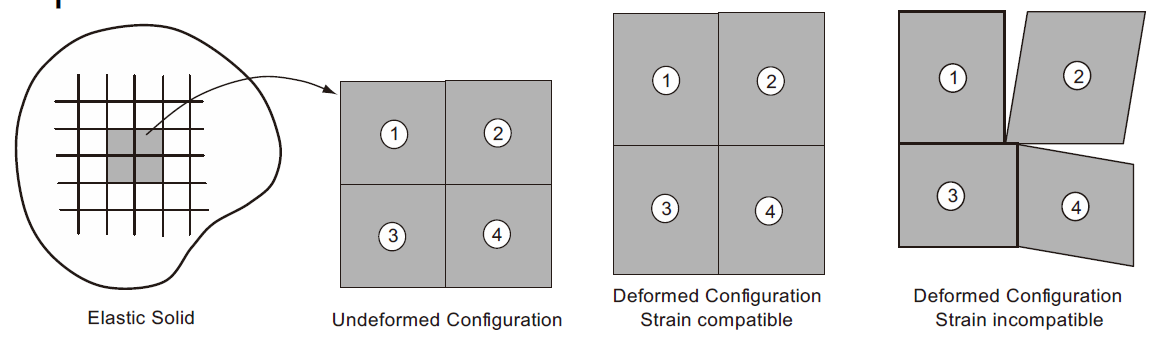
\includegraphics[width=0.6\textwidth]{image/012.png}
      \caption{Strain Compatibility}
      \label{fig:012}
    \end{figure}

    Six equations for the strain components are functions of only three displacement components. If six strain components are known, we have six equations for only three unknowns. There must be additional equations relate the six strain components, which are called \textbf{Strain Compatibility Equations}.\\

    \begin{equation}\label{eq:043}
      \left\{
      \begin{aligned}
        \frac{\partial^2 \epsilon_x}{\partial y^2} + \frac{\partial^2 \epsilon_y}{\partial x^2} &= \frac{\partial^2 \gamma_{xy}}{\partial x \partial y} \\
        \frac{\partial^2 \epsilon_y}{\partial z^2} + \frac{\partial^2 \epsilon_z}{\partial y^2} &= \frac{\partial^2 \gamma_{yz}}{\partial y \partial z} \\
        \frac{\partial^2 \epsilon_z}{\partial x^2} + \frac{\partial^2 \epsilon_x}{\partial z^2} &= \frac{\partial^2 \gamma_{zx}}{\partial z \partial x}
      \end{aligned}
      \right.
      , \quad
      \left\{
      \begin{aligned}
        2 \frac{\partial^2 \epsilon_x}{\partial y \partial z} &= \frac{\partial}{\partial x} \left( -\frac{\partial \gamma_{yz}}{\partial x} + \frac{\partial \gamma_{zx}}{\partial y} + \frac{\partial \gamma_{xy}}{\partial z} \right) \\
        2 \frac{\partial^2 \epsilon_y}{\partial z \partial x} &= \frac{\partial}{\partial y} \left( \frac{\partial \gamma_{yz}}{\partial x} - \frac{\partial \gamma_{zx}}{\partial y} + \frac{\partial \gamma_{xy}}{\partial z} \right) \\
        2 \frac{\partial^2 \epsilon_z}{\partial x \partial y} &= \frac{\partial}{\partial z} \left( \frac{\partial \gamma_{yz}}{\partial x} + \frac{\partial \gamma_{zx}}{\partial y} - \frac{\partial \gamma_{xy}}{\partial z} \right)
      \end{aligned}
      \right.
    \end{equation}

    The compatibility equation \cref{eq:043} can also be called as \textbf{Saint-Venant's compatibility equation}. In this equation, only three compatibility equations are independent. If the displacement components are single-valued, continuous functions, the strain components will automatically satisfy the compatibility equations.\\

\end{document}
